% Master thesis main document
% Author: Tommy O.
% Fall 2017

% -------------------------------------------------------------
% ---- DOCUMENT INITIALIZATION AND PACKAGE IMPORTS
% -------------------------------------------------------------

\documentclass[12pt, a4paper, twoside]{report} % 'twoside' when printing
\usepackage[utf8]{inputenc}				% UTF-8 input
\usepackage[english]{babel}				% Set language to english
\usepackage{blindtext}					% Use \Blinddocument or \blindmathpaper
\usepackage{graphicx}					% For graphics
\usepackage{fancyhdr}					% Fancy headers
\usepackage{hyperref}					% Internal and external hyperlinks
\usepackage{amsmath}					% Math from AMS
\usepackage{amsfonts}					% Fonts from AMS
\usepackage{amsthm}						% Theorems
\usepackage{amssymb}					% Symbols
\usepackage{enumitem}					% Enumeration
\usepackage{mathtools} 					% Bonus
\usepackage{color}						% Colors
\usepackage{booktabs}					% Professional tables
\usepackage{pdfpages}					% To include PDFs
\usepackage{parskip}					% Paragraph space
\usepackage{multicol}					% For multiple columns
\usepackage[sharp]{easylist}			% For easy lists
\usepackage{makeidx}					% For the index
\usepackage[linesnumbered,ruled]{algorithm2e}	% For algorithms
\usepackage{tikz-cd}					% For diagrams
\usepackage{listings}					% To include Python-code
\usepackage{etoolbox}					% To add symbol at end of examples
\usepackage[expansion=false]{microtype} % Fixes to make typography better
\usepackage[toc, page]{appendix} 		% To include appendices
%\usepackage[headings]{fullpage}		% Smaller margins
\usepackage[margin = 3cm, includehead, includefoot]{geometry}
%\usepackage[sc]{mathpazo}				% A nice font, alternative to CM
\usepackage{framed}						% To frame comments
\usepackage{multirow}					% For multiple rows in tables
\usepackage{afterpage}					% To insert blank pages
\usepackage{blindtext}

% -------------------------------------------------------------
% ---- PACKAGE SET UP
% -------------------------------------------------------------

%\usepackage[T1]{fontenc}				% Different font if wanted
\graphicspath{{figs/}}					% Path to graphics
\pagestyle{fancy}						% Set page headers to fancy

% PACKAGE SET UP -- algorithm2e
\SetKw{Continue}{continue}
\SetKw{Break}{break}
\SetKw{Yield}{yield}
\SetKw{In}{in}
\SetKw{Not}{not}
\newcommand\mycommfont[1]{\small\ttfamily{#1}}
\SetCommentSty{mycommfont}

% PACKAGE SET UP -- Theorems, equations, definitions setup
\newtheoremstyle{plainspaced}
{1em} % Space above
{1em} % Space below
{\em} % Body font
{} % Indent amount
{\bfseries} % Theorem head font
{.} % Punctuation after theorem head
{.5em} % Space after theorem head
{\thmname{#1}\thmnumber{ #2}\thmnote{ (#3)}} % Theorem head spec (can be left empty, meaning `normal')

\newtheoremstyle{definitionspaced}
{1em} % Space above
{1em} % Space below
{} % Body font
{} % Indent amount
{\bfseries} % Theorem head font
{.} % Punctuation after theorem head
{.5em} % Space after theorem head
{\thmname{#1}\thmnumber{ #2}\thmnote{ (#3)}} % Theorem head spec (can be left empty, meaning `normal')

\theoremstyle{plainspaced}
\newtheorem{theorem}{Theorem}[chapter]			% Theorem style
\newtheorem{lemma}[theorem]{Lemma}				% Lemma style
\newtheorem{problem}[theorem]{Problem}			% Lemma style
\newtheorem{proposition}[theorem]{Proposition}	% Proposition style

\theoremstyle{plainspaced}
\newtheorem{definition}[theorem]{Definition}	% Definition style
\theoremstyle{definitionspaced}
\newtheorem{example}[theorem]{Example}			% Definition style

% Add symbols at the end of example and definitions
\AtEndEnvironment{example}{\null\hfill $\lrcorner$}%
\AtEndEnvironment{definition}{\null\hfill $\lrcorner$}%

% Must run this command to use index
\makeindex

% Spacing in easylist items and rows/cols in diagrams
\newcommand{\listSpace}{-0.25em}
\newcommand{\diagramSpace}{3em}

% Set up for Python code
\usepackage{xcolor}
\definecolor{maroon}{cmyk}{0, 0.87, 0.68, 0.32}
\definecolor{halfgray}{gray}{0.55}
\definecolor{ipython_frame}{RGB}{207, 207, 207}
\definecolor{ipython_bg}{RGB}{255, 255, 255}
\definecolor{ipython_red}{RGB}{186, 33, 33}
\definecolor{ipython_green}{RGB}{0, 128, 0}
\definecolor{ipython_cyan}{RGB}{64, 128, 128}
\definecolor{ipython_purple}{RGB}{170, 34, 255}

\lstset{
	breaklines=true,
	%
	extendedchars=true,
	literate=
	{á}{{\'a}}1 {é}{{\'e}}1 {í}{{\'i}}1 {ó}{{\'o}}1 {ú}{{\'u}}1
	{Á}{{\'A}}1 {É}{{\'E}}1 {Í}{{\'I}}1 {Ó}{{\'O}}1 {Ú}{{\'U}}1
	{à}{{\`a}}1 {è}{{\`e}}1 {ì}{{\`i}}1 {ò}{{\`o}}1 {ù}{{\`u}}1
	{À}{{\`A}}1 {È}{{\'E}}1 {Ì}{{\`I}}1 {Ò}{{\`O}}1 {Ù}{{\`U}}1
	{ä}{{\"a}}1 {ë}{{\"e}}1 {ï}{{\"i}}1 {ö}{{\"o}}1 {ü}{{\"u}}1
	{Ä}{{\"A}}1 {Ë}{{\"E}}1 {Ï}{{\"I}}1 {Ö}{{\"O}}1 {Ü}{{\"U}}1
	{â}{{\^a}}1 {ê}{{\^e}}1 {î}{{\^i}}1 {ô}{{\^o}}1 {û}{{\^u}}1
	{Â}{{\^A}}1 {Ê}{{\^E}}1 {Î}{{\^I}}1 {Ô}{{\^O}}1 {Û}{{\^U}}1
	{œ}{{\oe}}1 {Œ}{{\OE}}1 {æ}{{\ae}}1 {Æ}{{\AE}}1 {ß}{{\ss}}1
	{ç}{{\c c}}1 {Ç}{{\c C}}1 {ø}{{\o}}1 {å}{{\r a}}1 {Å}{{\r A}}1
	{€}{{\EUR}}1 {£}{{\pounds}}1
}

%%
%% Python definition (c) 1998 Michael Weber
%% Additional definitions (2013) Alexis Dimitriadis
%% modified by me (should not have empty lines)
%%
\lstdefinelanguage{iPython}{
	morekeywords={access,and,break,class,continue,def,del,elif,else,except,exec,finally,for,from,global,if,import,in,is,lambda,not,or,pass,print,raise,return,try,while},%
	%
	% Built-ins
	morekeywords=[2]{abs,all,any,basestring,bin,bool,bytearray,callable,chr,classmethod,cmp,compile,complex,delattr,dict,dir,divmod,enumerate,eval,execfile,file,filter,float,format,frozenset,getattr,globals,hasattr,hash,help,hex,id,input,int,isinstance,issubclass,iter,len,list,locals,long,map,max,memoryview,min,next,object,oct,open,ord,pow,property,range,raw_input,reduce,reload,repr,reversed,round,set,setattr,slice,sorted,staticmethod,str,sum,super,tuple,type,unichr,unicode,vars,xrange,zip,apply,buffer,coerce,intern},%
	%
	sensitive=true,%
	morecomment=[l]\#,%
	morestring=[b]',%
	morestring=[b]",%
	%
	morestring=[s]{'''}{'''},% used for documentation text (mulitiline strings)
	morestring=[s]{"""}{"""},% added by Philipp Matthias Hahn
	%
	morestring=[s]{r'}{'},% `raw' strings
	morestring=[s]{r"}{"},%
	morestring=[s]{r'''}{'''},%
	morestring=[s]{r"""}{"""},%
	morestring=[s]{u'}{'},% unicode strings
	morestring=[s]{u"}{"},%
	morestring=[s]{u'''}{'''},%
	morestring=[s]{u"""}{"""},%
	%
	% {replace}{replacement}{lenght of replace}
	% *{-}{-}{1} will not replace in comments and so on
	literate=
	{á}{{\'a}}1 {é}{{\'e}}1 {í}{{\'i}}1 {ó}{{\'o}}1 {ú}{{\'u}}1
	{Á}{{\'A}}1 {É}{{\'E}}1 {Í}{{\'I}}1 {Ó}{{\'O}}1 {Ú}{{\'U}}1
	{à}{{\`a}}1 {è}{{\`e}}1 {ì}{{\`i}}1 {ò}{{\`o}}1 {ù}{{\`u}}1
	{À}{{\`A}}1 {È}{{\'E}}1 {Ì}{{\`I}}1 {Ò}{{\`O}}1 {Ù}{{\`U}}1
	{ä}{{\"a}}1 {ë}{{\"e}}1 {ï}{{\"i}}1 {ö}{{\"o}}1 {ü}{{\"u}}1
	{Ä}{{\"A}}1 {Ë}{{\"E}}1 {Ï}{{\"I}}1 {Ö}{{\"O}}1 {Ü}{{\"U}}1
	{â}{{\^a}}1 {ê}{{\^e}}1 {î}{{\^i}}1 {ô}{{\^o}}1 {û}{{\^u}}1
	{Â}{{\^A}}1 {Ê}{{\^E}}1 {Î}{{\^I}}1 {Ô}{{\^O}}1 {Û}{{\^U}}1
	{œ}{{\oe}}1 {Œ}{{\OE}}1 {æ}{{\ae}}1 {Æ}{{\AE}}1 {ß}{{\ss}}1
	{ç}{{\c c}}1 {Ç}{{\c C}}1 {ø}{{\o}}1 {å}{{\r a}}1 {Å}{{\r A}}1
	{€}{{\EUR}}1 {£}{{\pounds}}1,
	%
	literate=
	*{+}{{{\color{ipython_purple}+}}}1
	{-}{{{\color{ipython_purple}-}}}1
	{*}{{{\color{ipython_purple}$^\ast$}}}1
	{/}{{{\color{ipython_purple}/}}}1
	{^}{{{\color{ipython_purple}\^{}}}}1
	{?}{{{\color{ipython_purple}?}}}1
	{!}{{{\color{ipython_purple}!}}}1
	{\%}{{{\color{ipython_purple}\%}}}1
	{<}{{{\color{ipython_purple}<}}}1
	{>}{{{\color{ipython_purple}>}}}1
	{|}{{{\color{ipython_purple}|}}}1
	{\&}{{{\color{ipython_purple}\&}}}1
	{~}{{{\color{ipython_purple}~}}}1
	%
	{==}{{{\color{ipython_purple}==}}}2
	{<=}{{{\color{ipython_purple}<=}}}2
	{>=}{{{\color{ipython_purple}>=}}}2
	%
	{+=}{{{+=}}}2
	{-=}{{{-=}}}2
	{*=}{{{$^\ast$=}}}2
	{/=}{{{/=}}}2,
	%
	%   identifierstyle=\color{red}\ttfamily,
	commentstyle=\color{ipython_cyan}\ttfamily,
	stringstyle=\color{ipython_red}\ttfamily,
	keepspaces=true,
	showspaces=false,
	showstringspaces=false,
	%
	rulecolor=\color{ipython_frame},
	frame=single,
	frameround={t}{t}{t}{t},
	xleftmargin=5.5ex,
	framexleftmargin=7mm,
	tabsize=4,
	numbers=left,
	numberstyle=\tiny\color{halfgray},
	%
	%
	backgroundcolor=\color{ipython_bg},
	%   extendedchars=true,
	basicstyle=\scriptsize\ttfamily,
	keywordstyle=\color{ipython_green}\ttfamily,
	escapechar=\¢,escapebegin=\color{ipython_green},
}


\lstdefinelanguage{iPythonLarge}{
	morekeywords={access,and,break,class,continue,def,del,elif,else,except,exec,finally,for,from,global,if,import,in,is,lambda,not,or,pass,print,raise,return,try,while},%
	%
	% Built-ins
	morekeywords=[2]{abs,all,any,basestring,bin,bool,bytearray,callable,chr,classmethod,cmp,compile,complex,delattr,dict,dir,divmod,enumerate,eval,execfile,file,filter,float,format,frozenset,getattr,globals,hasattr,hash,help,hex,id,input,int,isinstance,issubclass,iter,len,list,locals,long,map,max,memoryview,min,next,object,oct,open,ord,pow,property,range,raw_input,reduce,reload,repr,reversed,round,set,setattr,slice,sorted,staticmethod,str,sum,super,tuple,type,unichr,unicode,vars,xrange,zip,apply,buffer,coerce,intern},%
	%
	sensitive=true,%
	morecomment=[l]\#,%
	morestring=[b]',%
	morestring=[b]",%
	%
	morestring=[s]{'''}{'''},% used for documentation text (mulitiline strings)
	morestring=[s]{"""}{"""},% added by Philipp Matthias Hahn
	%
	morestring=[s]{r'}{'},% `raw' strings
	morestring=[s]{r"}{"},%
	morestring=[s]{r'''}{'''},%
	morestring=[s]{r"""}{"""},%
	morestring=[s]{u'}{'},% unicode strings
	morestring=[s]{u"}{"},%
	morestring=[s]{u'''}{'''},%
	morestring=[s]{u"""}{"""},%
	%
	% {replace}{replacement}{lenght of replace}
	% *{-}{-}{1} will not replace in comments and so on
	literate=
	{á}{{\'a}}1 {é}{{\'e}}1 {í}{{\'i}}1 {ó}{{\'o}}1 {ú}{{\'u}}1
	{Á}{{\'A}}1 {É}{{\'E}}1 {Í}{{\'I}}1 {Ó}{{\'O}}1 {Ú}{{\'U}}1
	{à}{{\`a}}1 {è}{{\`e}}1 {ì}{{\`i}}1 {ò}{{\`o}}1 {ù}{{\`u}}1
	{À}{{\`A}}1 {È}{{\'E}}1 {Ì}{{\`I}}1 {Ò}{{\`O}}1 {Ù}{{\`U}}1
	{ä}{{\"a}}1 {ë}{{\"e}}1 {ï}{{\"i}}1 {ö}{{\"o}}1 {ü}{{\"u}}1
	{Ä}{{\"A}}1 {Ë}{{\"E}}1 {Ï}{{\"I}}1 {Ö}{{\"O}}1 {Ü}{{\"U}}1
	{â}{{\^a}}1 {ê}{{\^e}}1 {î}{{\^i}}1 {ô}{{\^o}}1 {û}{{\^u}}1
	{Â}{{\^A}}1 {Ê}{{\^E}}1 {Î}{{\^I}}1 {Ô}{{\^O}}1 {Û}{{\^U}}1
	{œ}{{\oe}}1 {Œ}{{\OE}}1 {æ}{{\ae}}1 {Æ}{{\AE}}1 {ß}{{\ss}}1
	{ç}{{\c c}}1 {Ç}{{\c C}}1 {ø}{{\o}}1 {å}{{\r a}}1 {Å}{{\r A}}1
	{€}{{\EUR}}1 {£}{{\pounds}}1,
	%
	literate=
	*{+}{{{\color{ipython_purple}+}}}1
	{-}{{{\color{ipython_purple}-}}}1
	{*}{{{\color{ipython_purple}$^\ast$}}}1
	{/}{{{\color{ipython_purple}/}}}1
	{^}{{{\color{ipython_purple}\^{}}}}1
	{?}{{{\color{ipython_purple}?}}}1
	{!}{{{\color{ipython_purple}!}}}1
	{\%}{{{\color{ipython_purple}\%}}}1
	{<}{{{\color{ipython_purple}<}}}1
	{>}{{{\color{ipython_purple}>}}}1
	{|}{{{\color{ipython_purple}|}}}1
	{\&}{{{\color{ipython_purple}\&}}}1
	{~}{{{\color{ipython_purple}~}}}1
	%
	{==}{{{\color{ipython_purple}==}}}2
	{<=}{{{\color{ipython_purple}<=}}}2
	{>=}{{{\color{ipython_purple}>=}}}2
	%
	{+=}{{{+=}}}2
	{-=}{{{-=}}}2
	{*=}{{{$^\ast$=}}}2
	{/=}{{{/=}}}2,
	%
	%   identifierstyle=\color{red}\ttfamily,
	commentstyle=\color{ipython_cyan}\ttfamily,
	stringstyle=\color{ipython_red}\ttfamily,
	keepspaces=true,
	showspaces=false,
	showstringspaces=false,
	%
	rulecolor=\color{ipython_frame},
	frame=single,
	frameround={t}{t}{t}{t},
	xleftmargin=5.5ex,
	framexleftmargin=7mm,
	tabsize=4,
	numbers=left,
	numberstyle=\scriptsize\color{halfgray},
	%
	%
	backgroundcolor=\color{ipython_bg},
	%   extendedchars=true,
	basicstyle=\footnotesize\ttfamily,
	keywordstyle=\color{ipython_green}\ttfamily,
	escapechar=\¢,escapebegin=\color{ipython_green},
}

% -------------------------------------------------------------
% ---- MISC SET UP
% -------------------------------------------------------------

% Custom mathematics commands
\newcommand{\norm}[1]{\left\lVert#1\right\rVert}
\newcommand{\abs}[1]{\left\lvert#1\right\rvert}
\newcommand*\conj[1]{\overline{#1}}
\DeclarePairedDelimiterX{\innerprod}[2]{\langle}{\rangle}{#1, #2}
\DeclareMathOperator{\coker}{coker}
\DeclareMathOperator{\im}{im}
\DeclareMathOperator{\coim}{coim}
\DeclareMathOperator{\lcm}{lcm}
\DeclareMathOperator{\diag}{diag}
\DeclareMathOperator{\C}{\mathbb{C}}
\DeclareMathOperator{\R}{\mathbb{R}}
\DeclareMathOperator{\Q}{\mathbb{Q}}
\DeclareMathOperator{\Z}{\mathbb{Z}}
\DeclareMathOperator{\N}{\mathbb{N}}
\DeclareMathOperator{\T}{\mathbb{T}}
\DeclareMathOperator{\F}{\mathcal{F}}
\DeclareMathOperator{\BO}{\mathcal{O}}
\DeclareMathOperator{\conv}{\ast}
\DeclareMathOperator{\argmin}{\operatorname{argmin}}
\DeclareMathOperator{\rank}{\operatorname{rank}}
\DeclareMathOperator{\GL}{\operatorname{GL}}
\DeclareMathOperator{\supp}{\operatorname{supp}}
\newcommand{\catname}[1]{{\normalfont\textsf{#1}}}
\newcommand{\Set}{\catname{Set}}
\newcommand{\VectR}{\catname{VectR}}
\newcommand{\VectZ}{\catname{ModZ}}
\newcommand{\Ab}{\catname{Ab}}
\newcommand{\FinAb}{\catname{FinAb}}

% A command to add a blank page
\newcommand\blankpage{%
	\null
	\newpage}

% Header set up with fancyhdr
\lhead[\nouppercase{\leftmark}]{\thepage} % EVEN, ODD
\rhead[\thepage]{\nouppercase{\rightmark}} % EVEN, ODD
\cfoot[]{}

\pagestyle{fancy}
\fancypagestyle{normal}{%
	% Header set up with fancyhdr
	\lhead[\nouppercase{\leftmark}]{\thepage} % EVEN, ODD
	\rhead[\thepage]{\nouppercase{\rightmark}} % EVEN, ODD
	\cfoot[]{}}
\fancypagestyle{noheadername}{%
	% Header set up with fancyhdr
	\lhead[]{\thepage} % EVEN, ODD
	\rhead[\thepage]{} % EVEN, ODD
	\cfoot[]{}}

% Declare first page in every chapter as 'fancy' pagestyle
\makeatletter
\renewcommand\chapter{\if@openright\cleardoublepage\else\clearpage\fi
	\thispagestyle{fancy}%
	\global\@topnum\z@
	\@afterindentfalse
	\secdef\@chapter\@schapter}
\makeatother

% Custom environment for comments
\newenvironment{comment}{\begin{framed} \footnotesize \textcolor{red}{\textbf{Comment.}}}{\end{framed} \normalsize}

\begin{document}
	
	% ---------------------------------------------------------
	% ---- Title page
	% ---------------------------------------------------------
	
	
\includepdf{cover/cover.pdf}
	\pagestyle{empty}
	\afterpage{\blankpage}
	\pagenumbering{roman}
	
	% ---------------------------------------------------------
	% ---- DOCUMENT INTRODUCTION
	% ---------------------------------------------------------
	
	\section*{Abstract}
	\pagestyle{normal}
	
	The abstract goes here.
	It should contain information about why the work was done, which problem that was solved, what was done, what is new, and how it was done.
	
	
	
	
	
%	\begin{comment}
%		From \cite{holst_scientific_nodate}
%		- Why did we do it? justify your work, put it into a broader context.
%		- what is the problem we are solving? (or which questions are answered)
%		- What did we do? list main results here.  take-home message.
%		- what is new? a brief comparison with state of the art.
%		- How did we do it? tools used, methods /theoretical tools
%	\end{comment}
%	
%	\begin{comment}
%		Guidelines from Nature
%		- 1-2 sentences with basic introduction to field, comprehensible to any scientist
%		- 2-3 sentences of more detailed background, comprehensible to scientists in related discliplines
%		- 1 sentence clearly stating the general problem
%		- 1 sentence summarizing the main result (``here we show...'')
%		- 2-3 sentences explaining main result in direct comparison to what was thought to be the case previously, or explain how main result adds to previous knowledge
%		- 1-2 sentences putting the result in general context
%		- 2-3 sentences to provide broader perspective
%	\end{comment}
%	
%	\begin{comment}
%		TODO: Write the abstract when everything else is finished.
%		See other theses on how to do this, or try the following:
%		(1) avoid notation if possible
%		(2) put the subject in context
%		(3) state results in non-technical language if possible
%		(4) mention technique if there is a new one
%		(5) never cite other papers in abstract.
%		see \url{https://www.maa.org/sites/default/files/pdf/students/Writing%20Abstracts.pdf}
%		or the book by Bodil
%	\end{comment}
	

	
	\vfill
	\section*{Acknowledgements}
	Write a acknowledgements.
	\vfill

	\setcounter{secnumdepth}{2}
	\setcounter{tocdepth}{1}
	\tableofcontents
	
	%\listoffigures
	
	%\listoftables
	
	\cleardoublepage
	\chapter*{Notation}
	\pagestyle{noheadername}
	\vspace*{-3em}
	%The following notation will be used throughout the thesis.
	\small 
	\begin{multicols}{2}
		\begin{easylist}[itemize]
			\ListProperties(Space*=\listSpace, Space=\listSpace, 
			Style1**=\bfseries, Style2*=, Hang=false, Progressive=1ex)
			
			# Groups
			## $\Z$ : Additive integers
			## $\Z_n = \Z / n \Z$ : Additive integers mod $n$
			## $\R$ : Additive reals
			## $T = \R / \Z$ : Additive reals mod $1$
			## $\T$ : Complex numbers $z$ with $\abs{z} = 1$
			## $GL(n, \Z)$ : Invertible matrices over $\Z$

			# Objects
			## $G, H$ : Abelian groups
			## $U, V$ : Unimodular matrices
			## $I_n$ : Identity matrix of size $n$
			
			# Binary operators
			%## $\innerprod{\cdot}{\cdot}$ : Inner product
			## $+$ : Addition
			## $\conv$ : Convolution
			## $\oplus$ : Direct sum
			
			# Relations
			## $\cong$ : Isomorphic
			## $>$ : Greater than
			## $\geq$ : Greater than or equal to
			

				
		\end{easylist}
	\end{multicols}
	\normalsize
	
	\section*{Abbreviations}
	\vspace*{-0.25em}
		\begin{easylist}[itemize]
			\ListProperties(Space*=\listSpace, 
			Space=\listSpace, 
			Style1**=\bfseries, 
			Style2*=, 
			Hang=false, 
			Progressive=1ex)
			## ML - Maximum likelihood
			## MAP - Maximum a posteriori
		\end{easylist}


	\cleardoublepage
	
	% ---------------------------------------------------------
	% ---- MAIN PART OF DOCUMENT
	% ---------------------------------------------------------
	
	\pagenumbering{arabic}
	\pagestyle{fancy}
	
	%\chapter{Notes}
	%\input{chapters/0_notes}
	
	\pagestyle{normal}
	\chapter{Introduction}
	\section{Introduction}
% write 1-2 pages -- brief history, overview of the field, what the thesis is about, what the goal of the thesis is, and what is new.
The introduction goes here.

\section{Chapter overview}

An overview of each chapter goes here.

\paragraph{Chapter 1 -- Introduction}
This chapter.

\paragraph{Chapter 2 -- Basic \LaTeX{}}
Some latex basics here.

\paragraph{Chapter 3 -- More \LaTeX{}}
Even more latex stuff here.

\paragraph{Appendices}
There is only one appendix, namely Appendix \ref{appendix:appendix_A}, which contains an example of how Python code can be included in a thesis.

	\chapter{Basic \LaTeX{}}
	\label{chapter:basic_latex}

% Paragraph descriping what the chapter is about
\blindtext

\section{A section with a definition and a theorem}
\label{sec:a_section_with_a_definition_and_a_theorem}

The above is a section. Here's a definition.

\begin{definition}[Conditional probability]
	\label{def:conditional_probability}
	The conditional probability of $A$ given $B$ is defined as
	\begin{equation*}
		P(A | B) = \frac{P(A \cap B)}{P(B)},
	\end{equation*}
	where $A \cap B$ denotes the intersection of $A$ and $B$.
\end{definition}

\begin{theorem}[Bayes theorem]
	Given $P(A | B)$, $P(A)$ and $P(B)$, we can compute $P(B | A)$ using 
	\begin{equation}
	\label{eqn:bayes_theorem}
	P(B | A) = \frac{P(A | B) P(B)}{P(A)}.
	\end{equation}
\end{theorem}
\begin{proof}
	Write $P(A \cap B)$ in two ways using the Definition \ref{def:conditional_probability} of conditional probability as follows.
	\begin{equation*}
		P(A \cap B) = P(A | B) P(B) \qquad P(B \cap A) = P(B | A) P(A)
	\end{equation*}
	The intersection is symmetric, meaning that $B \cap A = B \cap A$.
	Thus we can compare terms and write $P(A | B) P(B) = P(B | A) P(A)$, rearranging this gives Bayes theorem.
\end{proof}

Bayes theorem has many applications, such as the \emph{Naive Bayes Classifier}, which is a machine learning algorithm.
The classifier assigns a label to a piece of data, e.g. classifying an email as spam or not.
It's called ``naive'' since it assumes conditional independence.
Equation \eqref{eqn:bayes_theorem} has extensions when more variables are used.

\section{A section with an example}
In Section \ref{sec:a_section_with_a_definition_and_a_theorem} we gave a theorem, here's an example with a real world application.

\begin{example}[An example with numbers]
	Here's a little example with some numbers.
	\begin{align*}
		P(B | A) &= \frac{P(A | B) P(B)}{P(A)} \\
			 	 &= \frac{(0.3) (0.4)}{0.24} = \frac{0.12}{0.24} = \frac{1}{2}
	\end{align*}
	As you see, applications are everywhere.
\end{example}

\blindtext

\section{A section with a figure}
\blindtext
	\begin{figure}[ht!]
	\centering
	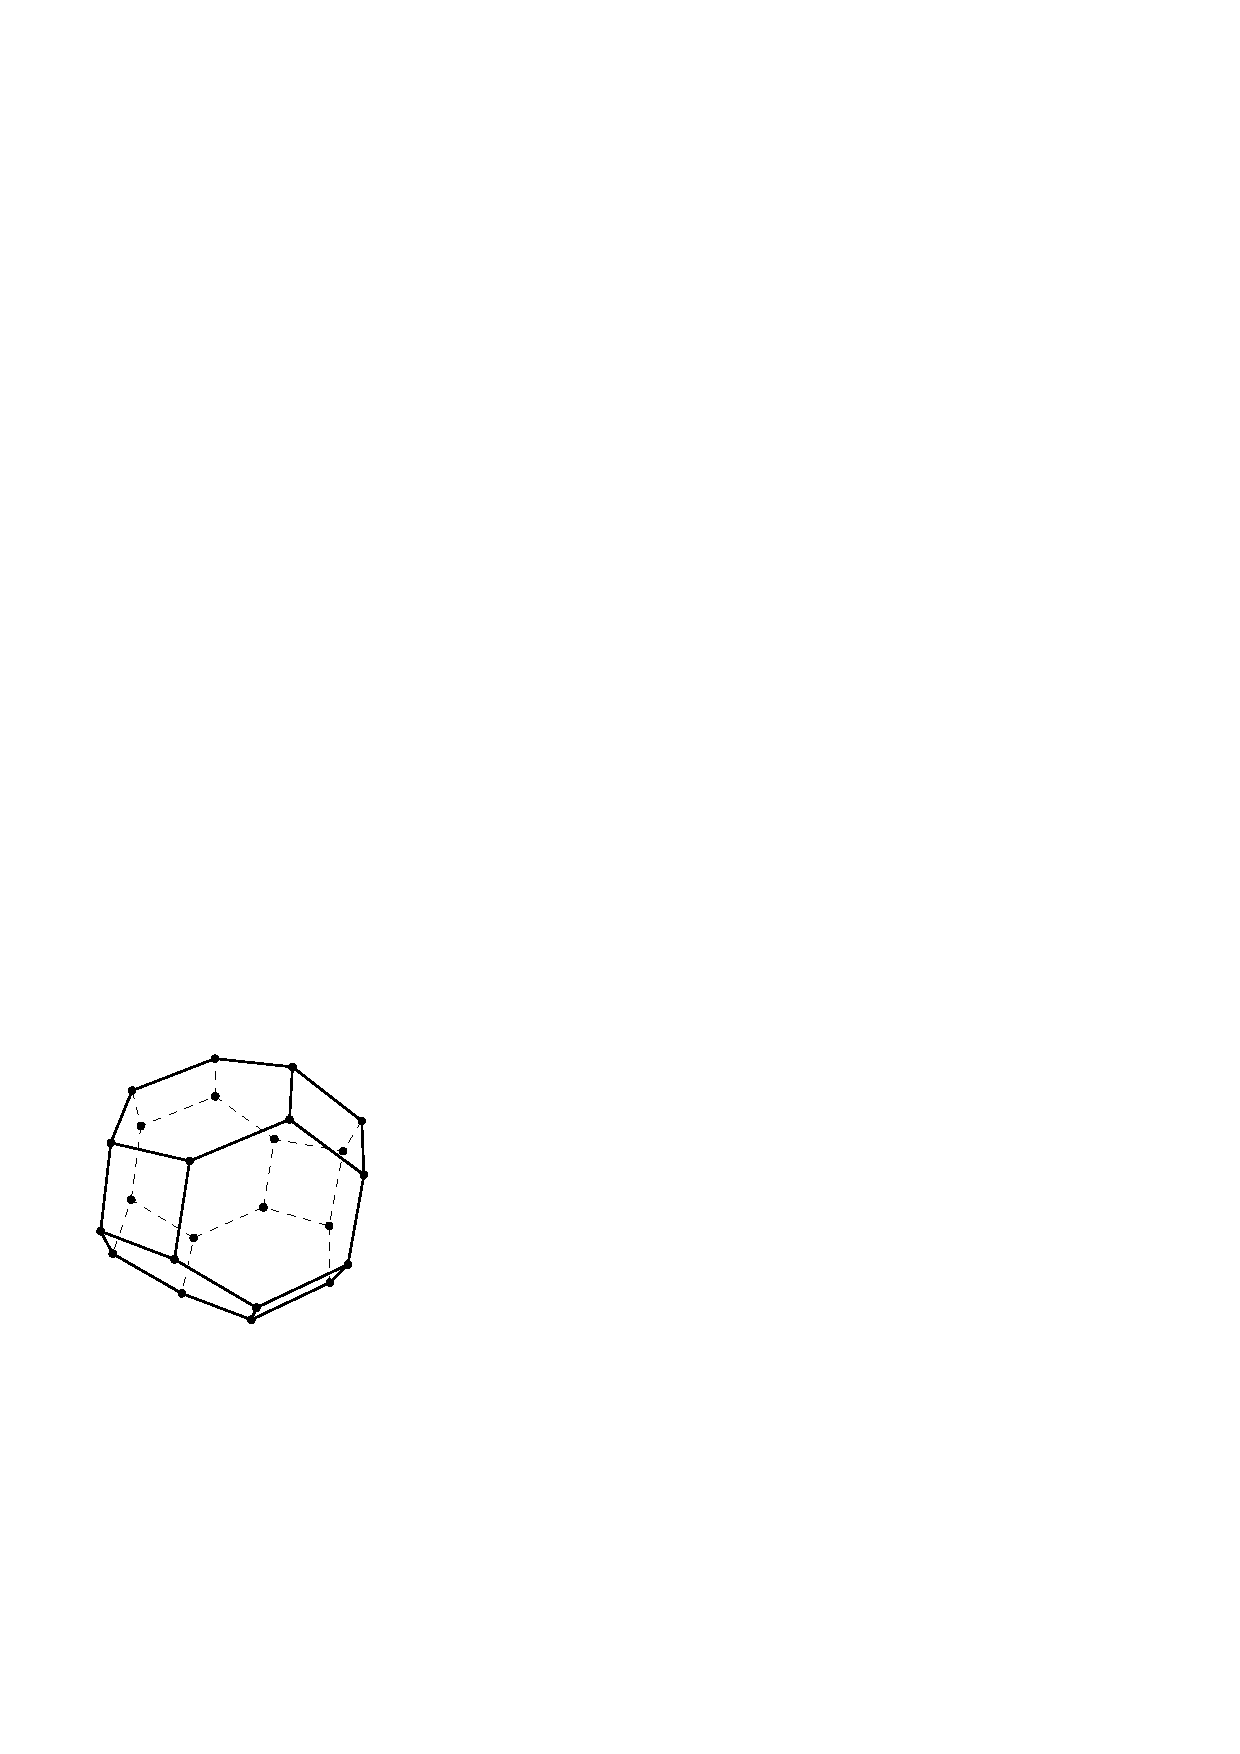
\includegraphics[width=0.3\linewidth]{figs/truncatedoctahedron}
	\caption{A pretty figure.}
	\label{fig:truncatedoctahedron}
	\end{figure}
\blindtext



	
	\chapter{Some more \LaTeX{}}
	\label{chapter:some_more_latex}

\section{References and lists}

Although \cite{strang_linear_1976} is a great introduction to linear algebra, \cite{roman_advanced_2005} presents the material in a more abstract way.

Here's a list of some linear algebra concepts.
\begin{easylist}[enumerate]
	\ListProperties(Space=\listSpace, Space*=\listSpace, Numbers1=a, Numbers2=r)
	
	# Linear algebra is about matrices and vectors.
	
	## The elements are usually numbers from $\R$ or $\C$.
	## Matrices are given by two indices, vectors by one.
	
	# Matrix multiplication is given by $y_i = \sum_j A_{ij} x_j$.
	
	# If $A = a_{ij}$, then the tranpose flips across the diagonal so that $A^T = a_{ji}$.
	The transpose is the adjoint, i.e. $\innerprod{Ax}{y} = \innerprod{x}{A^Ty}$.
\end{easylist}


Here's a different type of list.

\begin{easylist}[enumerate]
	\ListProperties(Space=\listSpace, Space*=\listSpace, Numbers=r, FinalMark={)})
	
	# Linear algebra is about matrices and vectors.
	
	## The elements are usually numbers from $\R$ or $\C$.
	## Matrices are given by two indices, vectors by one.

\end{easylist}

Here's a different type of list.

\begin{easylist}[itemize]
	\ListProperties(Space=\listSpace, Space*=\listSpace)
	
	# Linear algebra is about matrices and vectors.
	
	## The elements are usually numbers from $\R$ or $\C$.
	## Matrices are given by two indices, vectors by one.
	
	# Matrix multiplication is given by $y_i = \sum_j A_{ij} x_j$.
	
	# If $A = a_{ij}$, then the tranpose flips across the diagonal so that $A^T = a_{ji}$.
	The transpose is the adjoint, i.e. $\innerprod{Ax}{y} = \innerprod{x}{A^Ty}$.
\end{easylist}


\section{Algorithms}

Here's an algorithm.

\begin{algorithm}
	\label{algo:student_algorithm}
	\SetKwInOut{Input}{Input}
	\SetKwInOut{Output}{Output}
	%\DontPrintSemicolon % \PrintSemicolon

	\Input{Student $s$.}
	\Output{Inverse $s^{-1}$ such that $s \circ s^{-1} = s^{-1} \circ s = \text{Id}$.}
	\BlankLine
	
	\tcp{Morning.}
	Grab coffee\;
	\While{thesis not finished}{
		Read mathematics\;
		Write thesis\;
	}
	Relax for an hour\;
	\BlankLine
	\tcp{Evening.}
	\For{every friend $f \in F$}{
		Call $f$\tcp*{Give your friends a call.} \label{algline:call_friends}
		}
	Sleep\;
	\caption{Algorithm for a thesis.}
\end{algorithm}

Notice in Algorithm \ref{algo:student_algorithm} above that the student does in fact call his friends in line \ref{algline:call_friends}.

Here's some Python code.

\lstinputlisting[language = iPython, firstline=9]{./code/example_code/composition.py}


\section{title}
\blindtext

\subsection{title}
\blindtext

\subsubsection{title}
\blindtext

\subsubsection{title}
\blindtext

\section{title}
\blindtext
\subsection{title}
\blindtext

\subsubsection{title}
\blindtext

	
	% ---------------------------------------------------------
	% ---- INDEX
	% ---------------------------------------------------------
	
	%\printindex
	
	% ---------------------------------------------------------
	% ---- BIBLIOGRAPHY
	% ---------------------------------------------------------
	
	\bibliographystyle{apalike}%alpha, apalike is also good
	\bibliography{thesis_bibliography}
	
	% ---------------------------------------------------------
	% ---- APPENDICES
	% ---------------------------------------------------------
	
	\begin{appendices}
		\chapter{Example code}
		\label{appendix:appendix_A}

sdf



	\end{appendices}

\end{document}